%
% File: chap01.tex
% Author: Victor F. Brena-Medina
% Description: Introduction chapter where the biology goes.
%
\let\textcircled=\pgftextcircled
\chapter{State of the art}
\label{chap:stateOfTheArt}

\initial{R}everse Engineering is the process of unearthing information or architecture knowledge from any object, software or process and attempting to modify it and reconstruct it with or without new functionality using the information gained from tearing down the object granularly and the understanding of the process while analyzing its components and inner workings in detail.

%=======
\section{State of the art}
\label{sec:sec01}

\subsection{As of now}

To Reverse engineering an android application, a vast amount of knowledge  and understanding of all the technology involved in the development of an application is required. Not only is the Android development know-how a necessity but also the same levels of mastery in regards to the external components involved in the buildings phase. 

When hearing the term reverse engineering in the software development world, one most likely associates it to hacking or attacking an application, and while it is true that reverse engineering techniques are used by malicious hackers to find vulnerabilities or exploits to produce viruses, worms, or just malware in general.

Reverse engineering allows the  attacker to gain familiarity with the application and its inner workings to locate entry vectors or globally known vulnerabilities or bad practices that couldn't possible be known or found out while externally analyzing the application through testing.

There are many ways to preform reverse engineering , but the standard procedure always consists of obtaining an executable, disassemble it through some tool, scrutinize the output of the disassemble, preform memory mappings and other analysis techniques to view variables and attempt to obtain the original source code if successful. Even though the retrieval of the source code is not always necessary or even possible, tampering the variables and checking validations is still the best way to go in order to get an idea of what is hiding underneath all that binary code.

In an Android/Java environment the process of compiling a source code and getting an executable consists of the following.
\vspace{20px}

\begin{minted}
[bgcolor = lightGrey]
{bash}
.java files -> .class files -> one classes.dex file
\end{minted}

Preventing this attack has to be the main priority of any enterprise that wishes to avoid code modifications by third parties. Perhaps the most well known method for accomplishing this objective is a technique know as code obfuscation.

\subsection{What is Obfuscation}

In order to make potential attacker’s life harder and hide  code, what is needed is the ability to perform a process called obfuscation. Obfuscation is a deliberate act of creating code that is difficult for humans to understand. It can be done in various ways: renaming all variables and class names so that they are a gibberish, flattening the directory structure, moving methods between files, adding garbage code, changing strings to int/hex array equivalents etc. It is used in various languages. In Android Java the code is compiled, but in language like Javascript it’s sent with plain text - obfuscation might be a logical step there, too. \cite{scalacio}

Next up, a comparison between normal Java code and it's obfuscated counterpart.

\begin{minted}
[
frame=lines,
bgcolor = lightGrey,
linenos
]
{Java}
/*Example Java function*/

function NewObject(prefix)
{
    var count=0;
    this.SayHello=function(msg)
    {
          count++;
          alert(prefix+msg);
    }
    this.GetCount=function()
    {
          return count;
    }
}
var obj=new NewObject("Message : ");
obj.SayHello("You are welcome.");
\end{minted}

\begin{minted}
[
frame=lines,
bgcolor = lightGrey,
linenos
]
{Java}
/*Obfuscated Java code*/

var _0x888f=["\x53\x61\x79\x48\x65\x6C\x6C\x6F", "\x47\x65\x74\x43\x6F\x75\x6E\
x74","\x4D\x65\x73\x73\x61\x67\x65\x20\x3A\x20","\x59\x6F\x75\x20\x61\x72\x65\x
20\x77\x65\x6C\x63\x6F\x6D\x65\x2E"] ;function NewObject(_0xd6eex2){var _0xd6ee
x3=0;this[_0x888f[0]]=function(_0xd6eex4){_0xd6eex3++;alert(_0xd6eex2+_0xd6eex4
);};this[_0x888f[1]]=function(){return _0xd6eex3};}var obj= new NewObject(_0x8
88f[2]);obj.SayHello(_0x888f[3]);
\end{minted}
\vspace{20px}

In Android development there is a tool called ProGuard, which is responsible for obfuscation and optimization of the code. It has a wide variety of options, but we have to be careful which ones are chosen. ProGuard can sometimes break the code, if used improperly, it can cause errors in code that uses reflection or in libraries that do.

\subsection{ApkTool}
In order to start the reverse engeering process of an apk, the first step is to decompile the application, one way to accomplish this is through ApkTool. This CLI program carries within it the following features.
\begin{enumerate}
\item{Disassembling resources to nearly original form (including resources.arsc, classes.dex, 9.png. and XMLs)}
\item{Rebuilding decoded resources back to binary APK/JAR}
\item{Organizing and handling APKs that depend on framework resources}
\item{Smali Debugging (Removed in 2.1.0 in favor of IdeaSmali)}
\item{Helping with repetitive tasks}
\end{enumerate}

ApkTool is the most mainstream decompiler in android reverse engineering world, it is free , easy to use and well documented. 



\subsection{Analysis of Decompiled APKs}

Once an APK has been decompiled, a thorough analysis of the files generated must be made and that begins with an understanding of the most common files and directories found within a decompiled APK.
\begin{tikzpicture}[%
    scale=.7,
    grow via three points={one child at (0.5,-0.65) and
    two children at (0.5,-0.65) and (0.5,-1.1)},
    edge from parent path={(\tikzparentnode.south) |- (\tikzchildnode.west)}]
  \node [root] {unzipped}
    child { node [selected] {assets}
      child { node { crashlytics-build.properties}}
      child { node [selected] {fonts}}
      child { node [selected] {geofences}}
      child { node [selected] {geojson}}
      child { node [selected] {licenses}}
      child { node [selected] {splash}}
    }       
    child { node at (0,-3.5) [selected] {res}
      child { node [selected] {animator}}
      child { node [selected] {menu}}
      child { node [selected] {layout}}
      child { node [selected] {...}}
    }
    child { node at (0,-5.9) [selected] {lib}
      child { node [selected] {armeabi-v7a}}
    }
    child { node at (0,-7.0) [selected] {META-INF}
      child { node {CERT.RSA}}
      child { node {CERT.SF}}
      child { node {MANIFEST.MF}}
      child { node [selected] {services}}
    }
    child { node at (0,-9.5) {AndroidManifest.xml}}
    child { node at (0,-9.5) {build-data.properties}}
    child { node at (0,-9.5) {classes2.dex}}
    child { node at (0,-9.5) {classes3.dex}}
    child { node at (0,-9.5) {classes4.dex}}
    child { node at (0,-9.5) {classes.dex}}
    child { node at (0,-9.5) {resources.arsc}}
    ;
\end{tikzpicture}

As it can be seen the .apk format is really just a zipped archive with the binaries compiled, a breakdown of these directories is as follows.

\begin{enumerate}
\item{classes.dex}

Contains compiled application code, transformed into Dex bytecode. You might see more than one DEX file in your APK if you are using multidex to overcome the 65536 method limit. Beginning with Android 5.0 which introduced the ART runtime, these are compiled into OAT files by the ahead-of-time compiler at install time and put on the device’s data partition.
\item{res/}

This folder contains most XML resources (e.g. layouts) and drawables (e.g. PNG, JPEG) in folders with various qualifiers, like -mdpi and -hdpi for densities, -sw600dp or -large for screen sizes and -en, -de, -pl for languages. Please note that any XML files in res/ have been transformed into a more compact, binary representation at compile time, so you won’t be able to open them with a text editor from inside the APK.

\item{resources.arsc}

Some resources and identifiers are compiled and flattened into this file. It’s normally stored in the APK without compression for faster access during runtime. Compressing this file manually might seem like an easy win, but is actually not a good idea for at least two reasons. One, Play Store compresses any data for transfer anyway and two, having the file compressed inside the APK would waste system resources (RAM) and performance (especially app startup time).

\item{AndroidManifest.xml}

Similar to other XML resources, your application Manifest is transformed during compilation into a binary format. Play Store uses certain information contained in the AndroidManifest to decide if an APK can be installed on a device, checking against allowed densities or screen sizes and available hardware and features (such as a touchscreen). If you want to inspect those Manifest entries after compilation, you can use the aapt tool from the Android SDK:

\begin{minted}
[bgcolor = lightGrey]
{bash}
  $ apt dump badging your_app.apk
\end{minted}

\item{libs/}
This folder contains shared objects files (.so) which are mostly just C/C++ binaries that android accesses through JNI and must be included in the APK in order to take advantage of methods and calls not available in Java. This folder is sometimes not included in some decompiled apks, depends on the application.

\item{assets/}

This folder is used for any file assets that will not be used as Android-type resources. Most commonly this will be font files or game data, like levels and textures, as well as any other application data that you want to open directly as a file stream.
\item{META-INF/}

This folder is present in signed APKs and contains a list of all files in the APK with their signatures. The way signing in Android works currently is that it verifies the signatures against uncompressed file contents from the archive, one by one.
This has some interesting consequences. Because every entry in a ZIP file is stored separately, this means that you can change individual files’ compression level without re-signing. The signature verification will fail however if you remove any file from the archive after it is signed.
One more thing to note about how a signed APK is created is that the zipalign tool is used as the last stage of the build. If you change the contents of the archive by hand, normally you will have to re-sign, then zipalign before uploading the APK to the Play Store.

\end{enumerate}



% Actualmente $1/3$ del GDP Mundial esta concentrado en la web, sitios de comercio como Amazon.com, Ebay.com y Alibaba.com entre otros dominan el mercado comercial como nunca antes, los bancos han agilizado sus servicios atraves de apliaciones web y desde pequenos hasta grandes negocios son beneficiados por el uso de sistemas de informacion para aumentar su productividad.

% Con el aumento de la integracion de la web en nuestra vida cotidiana, en igual proporcion a subido los ataques a estos sistemas. El resguardo de la informacion, privacidad como tambien  protejerse de atacantes es una de los problemas mas grandes en servicios web en la actualidad. Asegurar que las aplicaciones web sean lo mas seguras posibles sea a convertido en una necesidad y esta dejando de ser un caracteristica atractiva de una aplicacion.

% Una de las formas de resguardar las aplicaciones es atraves de un proceso de pruebas, denominado penetration testing o Pentest. Este proceso de pruebas implica correr softwares de reconocimiento para obtener informacion de el objetivo, usar esta informacion para detectar fallas dentro de la aplicacion o por la periferia, para luego encontrar alguna vulnerabilidad que permita ingresar al sistema.

% Existen varias metodologias para un buen pentest. \cite{OWASP}

% \begin{enumerate}
% \item{OWASP testing guide}
% \item{PCI Penetration testing guide}
% \item{Penetration Testing Execution Standard}
% \item{NIST 800-115}
% \item{Penetration Testing Framework}
% \item{Information Systems Security Assessment Framework (ISSAF)}
% \item{Open Source Security Testing Methodology Manual (“OSSTMM”)}
% \end{enumerate}

% \section{Metodologias}

% Para poder conducir un pentest optimo, se debe recordar las cinco fases de analisis y recopilamiento de informacion. Resumidas a continuacion.

% \begin{enumerate}
% \item{Footprinting}
% \item{Scanning}
% \item{Exploit}
% \item{Payload}
% \item{Persitence}
% \end{enumerate}

% \subsection{Footprinting}
% La fase de footprinting consiste en buscar informacion publica de el objetivo a analisar, cuentas de linkedin, facebook, twitter, registros publics gubernamentales etc. Toda la informacion recopilada en esta fase puede ser muy valiosa en el futuro.

% \subsection{Scanning}
% La fase de escanear consiste en correr port scanners como Nmap para intentar enumarar las infraestrutura del objetivo, puertos publicos o privados, e intentar ver que servicios se albergan detras de estos junto con la version de ese software. Esta informacion es muy importante al momento de querer correr algun exploit sobre el objetivo.

% \subsection{Exploit}
% La fase de exploit consiste en analizar los datos recopilados en las dos fases anteriores e intentar encontrar una falla o vulnerabilidad que permita la ejecucion de codigo o extraccion de informacion no autorizada. Tambien es posible que al tener las versiones y servicios de los endpoints, encontrar una vulnerabrZilidad ya reportarda y que el objetivo no a actualizado.

% \subsection{Payload}

% La fase de payload consiste en que una vez encontrada la falla de seguridad o vulnerabilidad, usarla para conseguir acceso al sistema, y subir un script o un programa que ejecute el ataque deseado, dentros de estos ataques existen scripts malisios, malware, shells reversos etc.

% \subsection{Persistence}

% La fase de persistencia consiste en que una vez que se haya ejecutado el payload se debe instaurar una forma de acceso a la maquina sin pasar por la vulnerabilidad encontrada, mas bien levantar servicios o conectarse a servidores externos controlados por el atacante que permitan el facil acceso a la maquina atacada en caso de que la vulnerabilidad sea arreglada.



% \section{Herramientas}

% Para poder ejecutar un pentest eficiente es necesario el uso de herramientas que agilizen el proceso de obtencion de datos y colaboren en encontrar vulnerabilidades dentro de cualquier ambiente y aplicacion. A continuacion se presentara una coleccion de herramientas estandar en la industria de seguridad en informatica.

% \subsection{Scanners}

% \subsubsection{Vulnerabilidad}

% \begin{enumerate}
% \item{Nessus [Multi]} \\
% Nesus es un no de los scanners de vulnerabilidades mas usados por auditores y analistas de seguridad en el mundo, los usuarios pueden correr multiples scans, crear politicas de seguridad, generar scans por horario y generacion de reportes via email. Tambien integra con una gran mayoria de productos de seguridad y hardware usado por profesionales. 

% Permite el analisis en ambientes virtualizados y plataformas en la nube, como tambien deteccion de malware y el uso de botnets.

% \item{OpenVAS [Win, Unix]}

% El Open Vulnerability Assessment System (OpenVAS) es un framework compuesto de varios servicios y herramientas que ofrecen una comprensiva y poderosa plataforma de escanear y manejo de vulnerabilidades.

% El escaner esta acompanado por un constante flujo de mejoras de la NVT (Network Vulnerability Tests) con un total de 47.000 para Junio, 2016.

% \item{Core Impact [Win]}
% Core impact no es barato, pero es considerado ampliamente como la herramienta de explotación mas potente en la actualidad. Contiene una gran base de datos de exploits profesionales, tambien tiene mecanismos como hacer pivotes entre maquinas infectadas atraves de tuneles encriptados. 

% \item{Nexpose [Win,Unix]}


% \end{enumerate}

% \subsubsection{Web}

% \begin{enumerate}
% \item{Burp Suite [Multi]}
% Burp Suite es un servidor proxy que permite la captura y forward de paquetes para poder hacer crawling sobre una pagina para poder mapearla 
% \item{Nikto [Multi]}
% \item{w3af [Multi]}
% \item{WebScarab [Multi]}
% \item{sqlmap [Multi]}
% Permite correr conocidos strings de sql que permiten analizar si existen vulnerabilidades del tipo sql injection, su fuerte es blind sql injection pero permite tambien in-band sql injection y out-of-band.
% \item{skipfish [Multi]}
% \item{Acunetix WVS [Multi]}
% \item{AppScan [Multi]}

% \end{enumerate}

% \subsection{Sniffers}
% \begin{enumerate}
% \item{Wireshark [Multi]}
% Analizador de datos en la capa de red, permite la captura de paquetes y analisis de headers y metadata en un flujo de datos.
% \item{Cain and Abel [Win] }
% \item{Tcpdump [Multi] }
% \item{Ettercap [Multi] }
% Herramienta que permite montar ataques MitM (Man in the Middle) quedo descontinuada una vez que SSL se hizo mas popular e implementado a nivel global. Ultimamente ataques que permiten descarcatar el certificado SSL, a convertido a esta herramienta util nuevamente.
% \item{NetStumbler [Win] }
% \item{dsniff [Multi] }
% \item{NetworkMiner [Win] }
% \end{enumerate}

% \subsection{Exploitation}

% \begin{enumerate}
% \item{Metasploit [Multi]}
% Framework de exploits y payloads que permite el facil manejo de estas. Conocido como uno de los mejores frameworks del mundo para penetration testing. Permite generacion de scripts y persistencia atraves de pivots y herramientas propias del framework como Rail Gun.
% \item{w3af [Multi] }
% \item{Core Impact [Win] }
% \item{Social Engineer Toolkit [Multi] }
% \item{BeEF [Multi]}
% \end{enumerate}

% \subsection{Crackers}

% \begin{enumerate}
% \item{Aircrack-ngp [Unix]}
% El suite de Aircrack permite el analisis de redes Wifi en la banda 2.4 para atacar el estandar 802.11, esta herramienta permite escanear el aire por redes en el vecindario, captura e injeccion de paquetes, levantar access points falsos y crackear passwords de la red.
% \item{Cain and Abel [Win]}
% \item{John the Ripper [Multi]}
% John es la herramienta open source mas popular para crackear passwords a traves de fuerza bruta, permite generacion de diccionarios para atacar como tambien reemplazos por patron para aumentar aun mas el espectro de cobertura por los diccionarios.
% \item{THC Hydra [Unix]}
% Hydra es otro password cracker que recibe su nombre por su capacidad de generar threads para acelerar el proceso de fuerza bruta hacia servicios (1 cabeza de la hydra = un hilo de procesamiento). Permite ataques hacia servidores ssh, ftp, http, smtp entre otros.
% \item{ophcrack [Multi]}
% \item{Medusa [Unix]}


% \end{enumerate}

\section{System Specifications}

All programs and builds will be done under my own personal computer which is an ASUS ZenBook UX305, Processor Intel\textregistered Core \texttrademark 5Y10/5Y71 Processor, LPDDR3 1600 MHz SDRAM, 8 GB of RAM, 256GB SSD hard drive, Integrated Intel\textregistered HD Graphics 5300 on top of a Deepin OS 15.3 operating system.


% \label{subsec:subsec01}

% Begins a subsection.

% %A figures matrix.
% \begin{figure}[t!]
% \centering
% \begin{minipage}{3.3cm}
%     \centering
%     \subtop[]{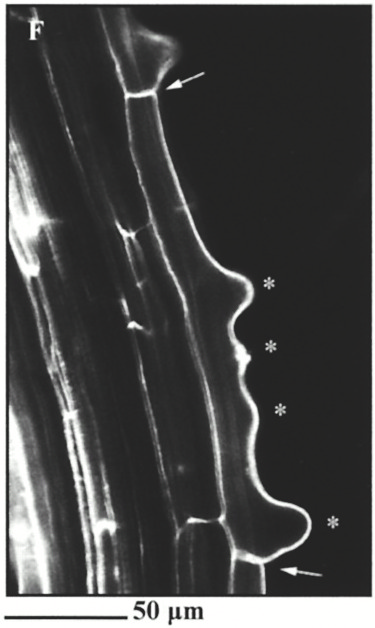
\includegraphics[height=0.28\textheight]{fig01/Nswellings}\label{sf:multiRH02a}}
% \end{minipage}
% \hspace{0.5cm}
% \begin{minipage}{3.3cm}
%     \centering
%     \subtop[]{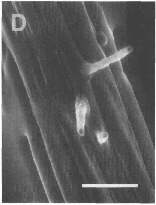
\includegraphics[height=0.27\textheight]{fig01/Mswellings}\label{sf:multiRH02b}}
% \end{minipage}
% \hspace{1.3cm}
% \begin{minipage}{3.3cm}
%     \centering
%     \subtop[]{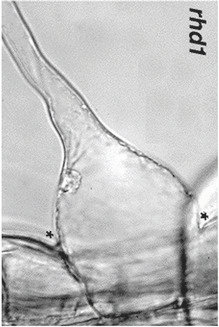
\includegraphics[height=0.27\textheight]{fig01/rhd1}\label{sf:multiRH02c}}
% \end{minipage}
% \\ \vspace{0.1cm}
% \begin{minipage}{10cm}
%     \centering
%     \subtop[]{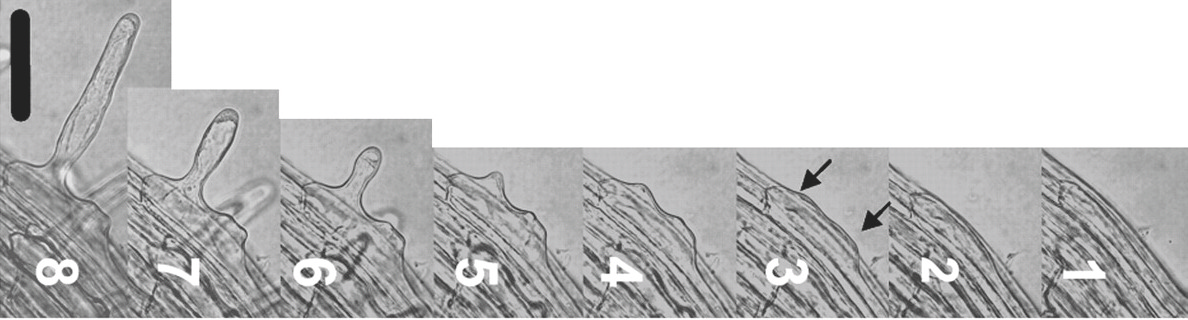
\includegraphics[height=0.145\textheight]{fig01/mutantrhd6}\label{sf:multiRH02d}}
% \end{minipage}
% \\ \vspace{0.1cm}
% \begin{minipage}{10cm}
%     \centering
%     \subtop[]{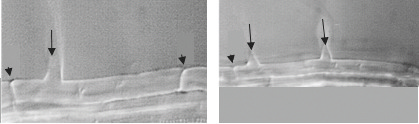
\includegraphics[height=0.16\textheight]{fig01/auxab}\label{sf:multiRH02e}}
% \end{minipage}
% \mycaption[Hair-forming mutant cells.]{(a) A mutant RH cell. Asterisks show multiple sites of RH initiation in a single root hair cell (indicated by the arrows). Figure reproduced from \cite{rigas01}. (b)~Hair-forming cell with three RH initiation locations. The bar represents $50\mu m$. Figure reproduced from \cite{massuci01}. (c) Large bump in mutant {\itshape rhd1}. Figure reproduced from \cite{griersonRH}. (d) Mutant overexpressing gene {\itshape ROP2}; from right-hand to left-hand, numbers indicate progressive snapshots at different times. RH initiation sites are indicated by the arrows. The bar represents $75\mu m$. Figure reproduced from~\cite{mjones01}. (e)~Mutants affected by auxin. On the left-hand side, RH site is farther away from the apical end (left arrow cap); on the right-hand side, multiple RH locations (arrows). Figure reproduced from~\cite{payne01}.}
% \label{fig:multiRH02}
% \end{figure}

% % A single figure
% \begin{figure}[t!]
% 	\centering
% 	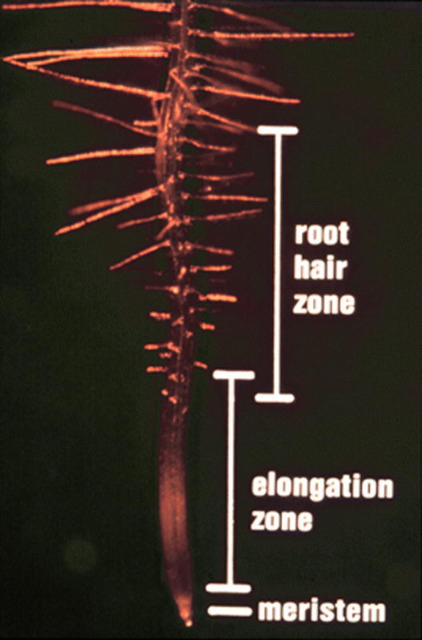
\includegraphics[height=0.35\textheight]{fig01/devepzones}
% 	\mycaption[Developmental zones of an Arabidopsis root.]{Developmental zones of an Arabidopsis root. Figure reproduced from \cite{griersonRH}.}
% 	\label{fig:RHP02}
% \end{figure}

%=========================================================